%% (Master) Thesis template
% Template version used: v1.4
%
% Largely adapted from Adrian Nievergelt's template for the ADPS
% (lecture notes) project.


%% We use the memoir class because it offers a many easy to use features.
\documentclass[11pt,a4paper,titlepage]{memoir}

%% Packages
%% ========

%% LaTeX Font encoding -- DO NOT CHANGE
\usepackage[OT1]{fontenc}

%% Babel provides support for languages.  'english' uses British
%% English hyphenation and text snippets like "Figure" and
%% "Theorem". Use the option 'ngerman' if your document is in German.
%% Use 'american' for American English.  Note that if you change this,
%% the next LaTeX run may show spurious errors.  Simply run it again.
%% If they persist, remove the .aux file and try again.
\usepackage[english]{babel}

%% Input encoding 'utf8'. In some cases you might need 'utf8x' for
%% extra symbols. Not all editors, especially on Windows, are UTF-8
%% capable, so you may want to use 'latin1' instead.
\usepackage[utf8]{inputenc}

%% This changes default fonts for both text and math mode to use Herman Zapfs
%% excellent Palatino font.  Do not change this.
\usepackage[sc]{mathpazo}

%% The AMS-LaTeX extensions for mathematical typesetting.  Do not
%% remove.
\usepackage{amsmath,amssymb,amsfonts,mathrsfs}

%% NTheorem is a reimplementation of the AMS Theorem package. This
%% will allow us to typeset theorems like examples, proofs and
%% similar.  Do not remove.
%% NOTE: Must be loaded AFTER amsmath, or the \qed placement will
%% break
\usepackage[amsmath,thmmarks]{ntheorem}

%% LaTeX' own graphics handling
\usepackage{graphicx}

%% We unfortunately need this for the Rules chapter.  Remove it
%% afterwards; or at least NEVER use its underlining features.
\usepackage{soul}

%% This allows you to add .pdf files. It is used to add the
%% declaration of originality.
\usepackage{pdfpages}

%% Some more packages that you may want to use.  Have a look at the
%% file, and consult the package docs for each.
\input{extrapackages}

%% Our layout configuration.  DO NOT CHANGE.
\input{layoutsetup}

%% Theorem environments.  You will have to adapt this for a German
%% thesis.
\input{theoremsetup}

%% Helpful macros.
\input{macrosetup}

%% Make document internal hyperlinks wherever possible. (TOC, references)
%% This MUST be loaded after varioref, which is loaded in 'extrapackages'
%% above.  We just load it last to be safe.
\usepackage[linkcolor=black,colorlinks=true,citecolor=black,filecolor=black]{hyperref}


%% Document information
%% ====================

\title{Algorithms for Pupil Detection}
\author{Anton Jakob Paris}
\thesistype{Semester Thesis}
\advisors{Dr.-Ing. Martin Weisenhorn }
\department{Image Processing and Computer Vision }
\date{23. February 2023}

\begin{document}

\frontmatter

%% Title page is autogenerated from document information above.  DO
%% NOT CHANGE.
\begin{titlingpage}
  \calccentering{\unitlength}
  \begin{adjustwidth*}{\unitlength-24pt}{-\unitlength-24pt}
    \maketitle
  \end{adjustwidth*}
\end{titlingpage}

%% The abstract of your thesis.  Edit the file as needed.
\begin{abstract}
In this thesis
\end{abstract}


%% TOC with the proper setup, do not change.
\cleartorecto
\tableofcontents
\mainmatter

%% Your real content!
% Some commands used in this file
\newcommand{\package}{\emph}

\chapter{Introduction}
\label{chap:introduction}
Pupil detection on images is a fundamental task with diverse applications in various fields, for example computer vision, human-computer interaction and biometric systems. Accurate and efficient pupil detection is crucial in tasks such as gaze tracking \cite{arar_robust_2017}, iris recognition \cite{wildes_iris_1997}, emotion recognition \cite{zheng_multimodal_2014} and medical diagnosis \cite{grubisic_natural_2014}.

Over the years, numerous algorithms and techniques have been proposed for pupil detection, each with strengths and limitations. However, most of these algorithms cannot perform well under various conditions. Consequently, finding a robust and efficient combination of algorithms for pupil detection is still an intriguing research problem. 
\section{Problem Statement}
\label{sec:problem_statement}
The problem of pupil detection discussed in this thesis is the optimal combination of algorithms for pupil detection, given the variability in imaging conditions, including variations in illumination, head poses, occlusions and quality of the images.

A single algorithm often fails to perform well under a wide span of conditions and lacks robustness and efficiency. Therefore this thesis aims to find a combination of algorithms that can perform well over a wide range of conditions without introducing machine learning, therefore, is independent of training data. 
\section{Motivation}
\label{sec:motivation}
The motivation behind this research is the lack of robustness and accuracy of current algorithms for pupil detection. Despite the extensive research on pupil detection no universal solution exists that can consistently handle the wide range of imaging conditions encountered in real-world scenarios. Therefore, exploring algorithmic combinations that can perform well under a wide range of conditions is a challenging and exciting research problem. 

Improving the pupil detection algorithm's performance can increase the precision and reliability of medical diagnosis, human-computer interaction and biometric systems. The benefit of exploring different approaches for pupil detection is the possibility of combining the strengths of different algorithms to achieve a more robust and efficient solution.

This thesis presents a comprehensive analysis of various algorithms for pupil detection and proposes a combination of algorithms. Through extensive experimentation and evaluation, the thesis aims to provide valuable insights and guidelines for researchers and practitioners working on pupil detection. Overall, this research seeks to contribute to developing more effective pupil detection systems that can operate reliably under varying imaging conditions, paving the way for improved applications and advancing the understanding of pupil detection. 



\chapter{Data Set}
\section{Labelled Pupils in the Wild (LPW)}
\subsection{Description}

The data set "Labelled Pupils in the Wild" \cite{zhang_max-planck-institut_nodate} or short LPW was created by the Max Plank Institution and and contains 66 high-quality, high-speed eye region videos for the development and evaluation of pupil detection algorithms. All videos are labeled with the center of the pupil. 22 participant's eye region with five different ethnicities, five different eye colors were recorded.  

The goal of the data set was to record samples of participants under conditions that are present in the reality. By having strong reflections, wearing glasses, wearing make up and so on the data set becomes a difficult challenge for pupil detection algorithms and a good evaluation of the algorithms is possible.


\begin{figure}[ht]
    \centering
    \begin{subfigure}{.30\textwidth}
      \centering
      \includegraphics[width=.9\linewidth]{plots/eye_dataset/eye1.png}

      \label{fig:ds1}
    \end{subfigure}%
    \begin{subfigure}{.30\textwidth}
      \centering
      \includegraphics[width=.9\linewidth]{plots/eye_dataset/eye2.png}

      \label{fig:ds2}
    \end{subfigure}%
    \begin{subfigure}{.30\textwidth}
      \centering
      \includegraphics[width=.9\linewidth]{plots/eye_dataset/eye3.png}

      \label{fig:ds3}
    \end{subfigure}
    \caption{three example frames from the LPW data set.}
    \label{fig:example_frame}
    \end{figure}

    \subsection{Procedure}
    The participants were asked to look at a moving red ball as it moved around. The recording location was randomly picked and was in and around several buildings. Each location was chosen once, creating a diverse range of real life situations. 

    For the recording a high-speed Pupil Pro head-mounted eye tracker was used that took 95 frames per second with a resolution of 640x480 pixels. With this frame rate even fast eye movements last through several frames making it more robust to detect the pupil.


    \begin{table}[h]
      \centering 
      \begin{minipage}{0.7\textwidth}
        \centering
        \begin{tabular}{|c|c|}
          \hline
          Location & Number of Videos \\
          \hline
          Outside & 34.3\% \\
          Inside & 65.7\% \\
          \hline
        \end{tabular}
        \caption{Location of recordings}
        \label{tab:location}
      \end{minipage}\hfill
      \begin{minipage}{0.7\textwidth}
        \centering
        \begin{tabular}{|c|c|}
          \hline
          Light source & Percentage of recordings \\
          \hline
          Natural light & 84.7\% \\
          Artificial light & 33.6\% \\
          \hline
        \end{tabular}
        \caption{Light Source of recordings}
        \label{tab:light_source}
      \end{minipage}
    \end{table}

    \subsection{Ground truth annotation}
    In many cases the pupil area has a clear boundary the center can be annotated easily. One or two points inside the pupil were manualy selected and used as seed points. From these point area with the same intensity value are extracted and used for annotation.  But in some difficult scenarios this method was not possibl because of strong noise over the pupil. In this case the additional information gained from the participants following a red fall with their eyes was used to create the labels. The frames then were manually annotated and this data was then used as calibration data to cross reference the center of the pupil with the position of the red ball. 
    
    The complete data set has labels for the center of the pupil for every frame.
    Given the ground truth annotation, it is possible to evaluate algorithms and compare them to each other.
    \subsection{Folder structure}
    The folder stands for the part, file number stands the participants and the file extension for the file type. The text file contains the ground truth annotation of the pupil center in x and y coordinates for each frame.
    
    The labels.ods file contains the information about the location, light source, vision aid used, prescription, nationality, eye color and gender. The README.txt file contains the information about the data set and the folder structure.
    
    The folder structure is shown in the following tree diagram.

    \dirtree{%
    .1 LPW/.
.2 labels.ods.
.2 README.txt.
.2 1.
.3 1.avi.
.3 1.txt.
.3 4.avi.
.3 4.txt.
.3 ....
.2 2.
.3 4.avi.
.3 4.txt.
.3 ....
.2 ....
.3 ....
.2 22. 
.3 ....
}
    \section{Eye characteristics}
    \subsection{Anatomy of the eye}
    The eye is surrounded by the \textbf{eye lid}. Its purpose is to shield the eye from debris and lubricate the eye by spreading tears over its surface with each blink. Then there are four different parts of the eye that matters for pupil detection. The white part of the eye is the \textbf{sclera} and is separated from the \textbf{iris} by the \textbf{limbus}.
    \begin{table}[h]
      \centering 
      \begin{minipage}{0.7\textwidth}
        \centering
        \begin{tabular}{|c|c|c|}
          \hline
          Name & Radius & Additional Information \\
          \hline
          Iris & 12 mm & in average\\
          Pupil & 2-9 mm & varies with light intensity\\
          \hline
        \end{tabular}
        \caption{Oversight iris and pupil radius}
        \label{tab:eye_char}
      \end{minipage}\hfill
    \end{table}
 

    The iris regulates the radius size of the \textbf{pupil} is and thereby regulates how much light comes through the pupil. The pupil is in the center of the iris and is the black part of the eye. The Darker the environment is, the larger the pupil radius. The Iris is colored and can be blue, green/hazle, brown, gray, amber and black. There are also other colors but they are in connection with health issues or genetic defects and play no role in this thesis. 

    The most important fact for pupil detection is that the iris, pupil and sclera have different brightness values. The pupil is the darkest area in the eye, the sclera is the brightest and the iris is in between. Depending on the color of the iris, the brightness value can vary.  Those characteristics are often used in pupil detection algorithms and will be discussed in the next chapter.
    \begin{figure}[ht]
      \centering
      \includegraphics[width=0.98\textwidth]{plots/eye_dataset/Various-characteristics-of-an-eye-and-its-iris-texture-7.png}
      \caption{Overview of the different parts of the eye.}
      \label{fig:eye_anatomy}
    \end{figure}
    There can also be reflections of the environment be seen in the eye. This reflection is called \textbf{purkinje reflection} and can temper with pupil detection algorithms accuracy and therefore is a challenge for pupil detection algorithms.


    \subsection{Image characteristics}
    \subsubsection{Histogram}
    When inspecting the histogram of a randomly chosen frame from the LPW data set, it can be seen that the histogram shows different peaks in different intensities. In this particular example it can be seen that the peak between 0 and 50 corresponds to the pupil it self. This can be be seen in figure \ref{fig:hist1} because when comparing both histograms the lowest peak stays unchanged. The intensity of the iris is therefore between 90 and 150.

    \begin{figure}[ht]
      \centering
      \includegraphics[width=0.9\textwidth]{plots/histogram_with_roi.png}
      \caption{Comparison histogram of the whole image and the region of interest.}
      \label{fig:hist1}
    \end{figure}

    The sclera is the brightest part of the eye but in this frame the skin intensity will be around the same magnitude as the sclera intensity. Subtracting the ROI from the original picture will result in a histogram almost only containing the skin and sclera. The histogram is therefore a strong tool for eye segmentation. 

    If there is more reflection on the pupil, the histogram will also change in its shape. The peak created by the pupil will shrink and flatten out. The mean of the histogram will increase as dark points are substituted by brighter points. This ultimately makes it hard for using a fixed threshold for segmentation. Using Histogram equalization increases the contrast of the image but stretches the peak into a wider intensity range. 

    Also interesting to inspect is one pixel row of the image with their intensity values. Here it can be observed that the pupil creates a valley in the intensity values. The reflection on the pupil generates a peak right after the valley. This can be seen in figure \ref{fig:row_intens}.
    \begin{figure}[ht]
      \centering
      \includegraphics[width=0.9\textwidth]{plots/row_intensity_valles.png}
      \caption{Plot of the intensity values of one pixel row.}
      \label{fig:row_intens}
    \end{figure}

    The x coordinate represents the pixel at this coordination and the y coordinate represents the intensity value of the pixel. 

    The conclusion is, that the histogram is a strong tool to gain insight information of the frame but can vary a lot depending on the environment, therefore adaptive algorithms have to be used. 
    

   
    \subsubsection{Gradients}
    As already shown in the previous subsection, the pupil creates a valley in the intensity values. This is also reflected in the gradient of the image. The gradient responds strongly to the change of intensity in the transition from the pupil to the iris. The orientation of the gradient points from the pupil towards the iris and can be of great help for edge detection. The gradient is calculated by using the Sobel operator. The Sobel operator is a discrete differentiation operator. It convolves the image with a differential kernel and therefore emphasizes regions with high spatial frequency. The Sobel operator will be discussed in a later chapter in more detail. But for know it's important to get an overview of the different characteristics of the eye.

    

    \begin{figure}[ht]
      \centering
      % First row: 3 images
      \begin{subfigure}{.33\textwidth}
        \centering
        \includegraphics[width=.9\linewidth]{plots/eye_dataset/roi.png}
        \caption{Image of ROI}
        \label{fig:roig}
      \end{subfigure}%
      \begin{subfigure}{.33\textwidth}
        \centering
        \includegraphics[width=.9\linewidth]{plots/eye_dataset/sx.png}
        \caption{Gradient in x\textbf{$G_{x}$}}
        \label{fig:sx}
      \end{subfigure}%
      \begin{subfigure}{.33\textwidth}
        \centering
        \includegraphics[width=.9\linewidth]{plots/eye_dataset/sy.png}
        \caption{Gradient in y \textbf{$G_{y}$}}
        \label{fig:sy}
      \end{subfigure}
      % Second row: 2 images
      \begin{subfigure}{.33\textwidth}
        \centering
        \includegraphics[width=.9\linewidth]{plots/eye_dataset/mag.png}
        \caption{Magnitude \textbf{$G$}}
        \label{fig:mag}
      \end{subfigure}%
      \begin{subfigure}{.33\textwidth}
        \centering
        \includegraphics[width=.9\linewidth]{plots/eye_dataset/direction.png}
        \caption{Orientation \textbf{$\theta$}}
        \label{fig:orientation}
      \end{subfigure}
      \caption{Plot of gradient characteristics of the ROI.}
      \label{fig:gradient}
      \end{figure}
      
      The gradient in x direction is shown in figure \ref{fig:sx} and the gradient in y direction is shown in figure \ref{fig:sy}. The magnitude of the gradient is shown in figure \ref{fig:mag} and the orientation of the gradient is shown in figure \ref{fig:orientation}. Depending on the environment, the gradient itself could already sufficient for pupil detection. In image processing the gradient is often used for edge detection and all sorts of different filters. Used correctly it can be very powerful. The magnitude is calulated by the following formula: 

      \begin{equation}
        \label{eq:magnitude}
        \begin{split}
          G = \sqrt{G_x^2 + G_y^2}
        \end{split}
      \end{equation}
      Because we have the gradient in x and y direction, we can calculate the orientation of the magnitude by using the following formula: 
      \begin{equation}
        \label{eq:orientation}
        \begin{split}
          \theta  = \arctan{\frac{G_y}{G_x}}
        \end{split}
      \end{equation}
      The orientation is calculated in radians and can be converted to degrees by multiplying it with $\frac{180}{\pi}$. The orientation is perpenticular to the edge and points in the direction of the gradient. Because the pupil is darker than the iris, the gradient points from the pupil to the iris. 

    \subsubsection{Noise}
      In the data set there are different kind of noise. The most common noise is the noise created by the camera. This noise is called \textbf{Gaussian noise}. Gaussian noise is a statistical noise having a probability density function equal to that of the normal distribution, which is also known as the Gaussian distribution. The noise is created by the camera and is therefore not dependent on the environment. The noise is therefore not a problem for the pupil detection algorithm.

      Considering that the goal is to detect the pupil there can also be other noise that can be problematic. \textbf{Reflection} of the environment can have an impact on the accuracy of the algorithm and destroy information about the pupil. Also the \textbf{eyelashes} can be problematic. They are very dark and therefore temper with the edges of the pupil and iris. Especially when the eyelashes are in front of the pupil. Also if make up is used. 

      Another Noise term can be that the eye is not constantly open. The \textbf{eyelid} can cover parts of the pupil or even the whole pupil. Then also glasses or lenses can add noise to the image. 
\chapter{Theory}
\section{Algorithms}
This chapter will take a look at commonly used algorithms in image processing for edge detection, identifying areas of interest and applying them onto pupil detection. At first the algorithms will be discussed and analyzed on possible use cases, individual strengths and weaknesses. To show the nature of the algorithm, the same preprocessed images from the LPW data set are used and therefore it is possible to showcase the results and compare them. 

\subsection{Fundamental notation}\label{subsec:funda}
Thru out this thesis the following notation is used to descripe the algorithms.
The image with intensity level $I$ is a function 

$f(x,y): \mathbb{\mathbb{N_0} }^2 \rightarrow \mathbb{\mathbb{N_0}}$, where $f(x,y)$ is the intensity $I \in $ [$0,255$] at position $(x,y)$

In image processing there the coordinate system is defined different than in mathematics. The origin is in the upper left corner and the x-axis is pointing to down vertically. The y axis is pointing to the right horizontally. this is shown in figure \ref{fig:coordsystem}.

\begin{figure}[h]
    \centering

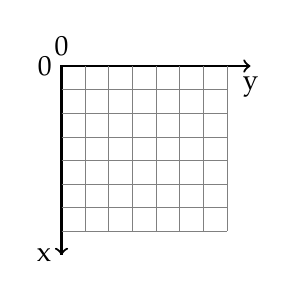
\begin{tikzpicture}[x=0.3cm,y=-0.3cm]
    
    % Draw the x-axis
    \draw[->,thick] (0,8) -- (0,0) -- (8,0) node[below] {y};
    % Draw the y-axis
    \draw[->,thick] (0,0) -- (0,8) node[left] {x};
    % Label the origin
    \node at (0,0) [left] {0};
    \node at (0,0) [above] {0};
    \foreach \x in {1,2,...,7}
    \draw[gray, very thin] (\x,0) -- (\x,7);
  \foreach \y in {1,2,...,7}
    \draw[gray, very thin] (0,\y) -- (7,\y);
  \end{tikzpicture}

    \caption{Coordinate system used in image processing.}
    \label{fig:coordsystem}
\end{figure}

Also important to note it that the image is a discrete function, therefore each intensity value $I$ comes with an quantization error. This is also the case when using an algorithm on the intensity values of the image. So it is not possible to have an exact result, it is always an approximation of the real result.

\subsubsection{Relationship between pixels}
One also important theory in this thesis will be based on relationship between pixels. In this subsection the terms \textbf{neighborhood}, \textbf{adjacency}, \textbf{connectivity}, \textbf{region} and \textbf{boundaries} will be introduced and visualized, so that they can be used in the following chapters. 

\paragraph{Neighborhood}
A pixel $P$ at location $(x,y)$ has two vertical neighbor pixels and two horizontal neighbor pixels in a 2D image. These neighbors are defined as $N_4(P)$ with coordinates: 
\begin{equation}
        N_4(P) = \{(x,y+1),(x,y-1),(x+1,y),(x-1,y)\}
\end{equation}
A pixel $P$ at location $(x,y)$ has four diagonal neighbor pixels in a 2D image. These neighbors are defined as $N_D(P)$ with coordinates:
\begin{equation}
    N_D(P) = \{(x+1,y+1),(x+1,y-1),(x-1,y+1),(x-1,y-1)\}
\end{equation}

Adding the neighbors from $N_4(P)$ and $N_D(P)$ results in the 8-neighborhood $N_8(P)$ of pixel $P$ with coordinates:
\begin{equation}
    N_8(P) = N_4(P) \cup N_D(P)
\end{equation}


    \begin{figure}[ht]
        \centering
        \begin{subfigure}[b]{0.23\textwidth}
            \centering
            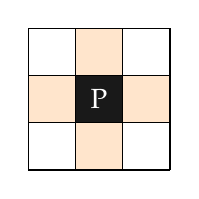
\begin{tikzpicture}[scale=0.6]
                \draw (0,0) grid (3,3);
                \filldraw[fill=orange!20] (1,0) rectangle (2,1);
                \filldraw[fill=orange!20] (1,2) rectangle (2,3);
                \filldraw[fill=orange!20] (0,1) rectangle (1,2);
                \filldraw[fill=orange!20] (2,1) rectangle (3,2);
                \filldraw[fill=black!90] (1,1) rectangle (2,2);
                \node[white] at (1.5,1.5) {P};
            \end{tikzpicture}
            \caption{$N_4(P)$}
            \label{fig:n_4}
        \end{subfigure}%
        \begin{subfigure}[b]{0.23\textwidth}
            \centering
            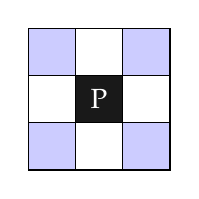
\begin{tikzpicture}[scale=0.6]
                \draw (0,0) grid (3,3);
                \filldraw[fill=blue!20] (0,3) rectangle (1,2);
                \filldraw[fill=blue!20] (2,0) rectangle (3,1);
                \filldraw[fill=blue!20] (0,0) rectangle (1,1);
                \filldraw[fill=blue!20] (2,2) rectangle (3,3);
                \filldraw[fill=black!90] (1,1) rectangle (2,2);
                \node[white] at (1.5,1.5) {P};
            \end{tikzpicture}
            \caption{$N_D(P)$}
            \label{fig:n_d}
        \end{subfigure}%
        \begin{subfigure}[b]{0.23\textwidth}
            \centering
            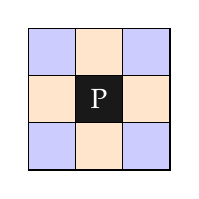
\begin{tikzpicture}[scale=0.6]
                \draw (0,0) grid (3,3);
                \filldraw[fill=blue!20] (0,3) rectangle (1,2);
                \filldraw[fill=blue!20] (2,0) rectangle (3,1);
                \filldraw[fill=blue!20] (0,0) rectangle (1,1);
                \filldraw[fill=blue!20] (2,2) rectangle (3,3);
                \filldraw[fill=orange!20] (1,0) rectangle (2,1);
                \filldraw[fill=orange!20] (1,2) rectangle (2,3);
                \filldraw[fill=orange!20] (0,1) rectangle (1,2);
                \filldraw[fill=orange!20] (2,1) rectangle (3,2);
                \filldraw[fill=black!90] (1,1) rectangle (2,2);

                \node[white] at (1.5,1.5) {P};
            \end{tikzpicture}
            \caption{$N_8(P)$}
            \label{fig:n_8}
        \end{subfigure}%
        \caption{3 different neighborhoods of pixel $P$ at location $(x,y)$.}
        \label{fig:neighborhoods}
    \end{figure}


\paragraph*{Adjacency} Mainly there are three types of adjacent pixels in a 2D image. Let $V$ be the set of intensity values used to define adjacency. Depending on the intensity range of the image, it's possible to define different subsets of $V$, containing the intensity values that are considered as adjacent in the neighborhood. In a binary image $V$ is often defined as $V$ = $\{1\}$, where $0$ stands for background and $1$ for foreground (This can also be considered a binary mask). In a grayscale image $V$ can be defined as any subeset of the intensity range. In this thesis the intensity range is $V$ = $\{0,1,2,...,255\}$.

To keep it simple, the following explanations will be based on a binary image with $V$ = $\{1\}$. Let define $P$ as a pixel at location $(x,y)$ and $Q$ as a pixel at location $(x',y')$. $P$ and $Q$ are considered adjacent if $Q$ is in the neighborhood of $P$ and $f(Q)$ is in $V$. These are the three adjacency types:

\begin{itemize}
    \item 4-adjacency, if $Q \in N_4(P) and f(Q) \in  V$: The pixels that are directly above, below, left and right of the pixel.
    \item 8-adjacency, if $Q \in N_8(P) and f(Q) \in  V$: The pixels that are directly above, below, left, right and the pixels that are diagonally adjacent to the pixel.
\end{itemize}
\begin{equation*}
    \bullet \text{ m-adjacency} \begin{cases}
   \text{if } Q \in N_4(P) \text{ and } f(Q) \in  V \\
    Q \in N_D(P) \text{ and } N_D(P)  \cap N_4(Q) \text{ has no intensities} \in  V
    \end{cases}
    \end{equation*}


    \begin{figure}[ht]
        \centering
        \begin{subfigure}{0.40\textwidth}
            \centering
            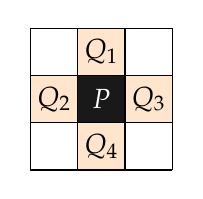
\begin{tikzpicture}[scale=0.6]
                \draw (0,0) grid (3,3);
                \filldraw[fill=orange!20] (1,0) rectangle (2,1);
                \filldraw[fill=orange!20] (1,2) rectangle (2,3);
                \filldraw[fill=orange!20] (0,1) rectangle (1,2);
                \filldraw[fill=orange!20] (2,1) rectangle (3,2);
                \filldraw[fill=black!90] (1,1) rectangle (2,2);


                \node[white] at (1.5,1.5) {$P$};
                \node at (1.5,2.5) {$Q_1$};
                \node at (0.5,1.5) {$Q_2$};
                \node at (2.5,1.5) {$Q_3$};
                \node at (1.5,0.5) {$Q_4$};




            \end{tikzpicture}
            \caption{4-adjacency}
            \label{fig:a_4}
        \end{subfigure}%
        \begin{subfigure}{0.40\textwidth}
            \centering
            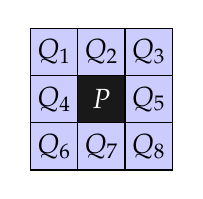
\begin{tikzpicture}[scale=0.6]
                \draw (0,0) grid (3,3);
                \filldraw[fill=blue!20] (0,3) rectangle (1,2);
                \filldraw[fill=blue!20] (2,0) rectangle (3,1);
                \filldraw[fill=blue!20] (0,0) rectangle (1,1);
                \filldraw[fill=blue!20] (2,2) rectangle (3,3);
                \filldraw[fill=blue!20] (1,0) rectangle (2,1);
                \filldraw[fill=blue!20] (1,2) rectangle (2,3);
                \filldraw[fill=blue!20] (0,1) rectangle (1,2);
                \filldraw[fill=blue!20] (2,1) rectangle (3,2);
                \filldraw[fill=black!90] (1,1) rectangle (2,2);
                \node[white] at (1.5,1.5) {$P$};
                \node at (0.5,0.5) {$Q_6$};
                \node at (1.5,0.5) {$Q_7$};
                \node at (2.5,0.5) {$Q_8$};
                \node at (0.5,1.5) {$Q_4$};
                \node at (2.5,1.5) {$Q_5$};
                \node at (0.5,2.5) {$Q_1$};
                \node at (1.5,2.5) {$Q_2$};
                \node at (2.5,2.5) {$Q_3$};
            \end{tikzpicture}
            \caption{$8-adjacency$}
            \label{fig:a_8}
        \end{subfigure}%

        \caption{3 different neighborhoods of pixel $P$ at location $(x,y)$.}
        \label{fig:adjacency}
    \end{figure}
\paragraph{Connectivity}
The connectivity of point $P$ is a set of points that can be reached in $n$ steps with a given adjacency type and intensity set $V$. If point $P$ is connected with $Q$ then there exist a path (or curve) from $P$ to $Q$ that consists of a sequence of distinct pixels with coordinates 
\begin{equation*}
    (x_0,y_0),(x_1,y_1),...,(x_n,y_n), \text{ where $n$ is the lenght of the path.}
\end{equation*}
If the path is closed then $(x_0,y_0) = (x_n,y_n)$
\paragraph{Region}
Let's define $R$ as an subset of pixels in an image. $R$ is a region if all points $\in R$ are a connected set, meaning that all points in $R$ are connected with each other and therefore form a region. This does not mean that the path connecting all points is closed.  Two regions can be adjacent to each other, if their union again forms a connected set. 

\paragraph{Boundary}
The outer boundary of a region $R$ is the set of pixels not in $R$ that are adjacent to pixels in $R$. In the definition of a boundary, the adjacency type is important. As a rule of thumb to define the boundary, the 8-adjacency is used. One important property of the outer boundary is, that it is a closed path. The inner boundary is the set of pixels that are in $R$ but are adjacent to at least one pixel that is not in $R$ and again the 8-adjacency is used. The inner boundary is not a closed path. 

\begin{figure}[ht]
    \centering
    \begin{subfigure}{0.40\textwidth}
        \centering
        \begin{tikzpicture}
            \matrix [matrix of nodes, nodes in empty cells, nodes={minimum width=1.5em, minimum height=1.5em, draw, thick, anchor=center}, column sep=-\pgflinewidth, row sep=-\pgflinewidth] (M)
            {
                |[fill=gray!20]| & |[fill=gray!20]| & |[fill=gray!20]| & |[fill=gray!20]| & |[fill=gray!20]| & |[fill=gray!20]| & |[fill=gray!20]| \\
                |[fill=gray!20]| & |[fill=gray!20]| & |[fill=gray!20]| & |[fill=red!20]|1 & |[fill=red!20]|1 & |[fill=gray!20]| & |[fill=gray!20]| \\
                |[fill=gray!20]| & |[fill=gray!20]| & |[fill=gray!20]| & |[fill=gray!20]| & |[fill=red!20]|1 & |[fill=red!20]|1 & |[fill=gray!20]| \\
                |[fill=gray!20]| & |[fill=gray!20]| & |[fill=gray!20]| & |[fill=gray!20]| & |[fill=gray!20]| & |[fill=red!20]|1 & |[fill=gray!20]| \\
                |[fill=gray!20]| & |[fill=red!20]|1 & |[fill=gray!20]| & |[fill=gray!20]| & |[fill=red!20]|1 & |[fill=red!20]|1 & |[fill=gray!20]| \\
                |[fill=gray!20]| & |[fill=red!20]|1 & |[fill=red!20]|1 & |[fill=red!20]|1 & |[fill=red!20]|1 & |[fill=gray!20]| & |[fill=gray!20]| \\
                |[fill=gray!20]| & |[fill=gray!20]| & |[fill=gray!20]| & |[fill=gray!20]| & |[fill=gray!20]| & |[fill=gray!20]| & |[fill=gray!20]| \\
            };
            
            \draw [thick] (M-1-1.north west) rectangle (M-7-7.south east);
        \end{tikzpicture}
        
        
            
        \caption{region $R$}
        \label{fig:region}
    \end{subfigure}%
    \begin{subfigure}{0.40\textwidth}
        \centering
        \begin{tikzpicture}
            \matrix [matrix of nodes, nodes in empty cells, nodes={minimum width=1.5em, minimum height=1.5em, draw, thick, anchor=center}, column sep=-\pgflinewidth, row sep=-\pgflinewidth] (M)
            {
                |[fill=gray!20]| & |[fill=gray!20]| & |[fill=red!20]| & |[fill=red!20]| & |[fill=red!20]| & |[fill=red!20]| & |[fill=gray!20]| \\
                |[fill=gray!20]| & |[fill=gray!20]| & |[fill=red!20]| & 1 & 1 & |[fill=red!20]| & |[fill=red!20]| \\
                |[fill=gray!20]| & |[fill=gray!20]| & |[fill=red!20]| & |[fill=red!20]| & 1 & 1 & |[fill=red!20]| \\
                |[fill=red!20]| & |[fill=red!20]|& |[fill=red!20]| & |[fill=red!20]| & |[fill=red!20]| & 1 & |[fill=red!20]| \\
                |[fill=red!20]| & 1 & |[fill=red!20]| & |[fill=red!20]| & 1 & 1 & |[fill=red!20]| \\
                |[fill=red!20]| & 1 & 1 & 1 & 1 & |[fill=red!20]| & |[fill=red!20]| \\
                |[fill=red!20]| & |[fill=red!20]| & |[fill=red!20]| & |[fill=red!20]| & |[fill=red!20]| & |[fill=red!20]| & |[fill=gray!20]| \\
            };
        
            \draw [thick] (M-1-1.north west) rectangle (M-7-7.south east);
        \end{tikzpicture}
        
        \caption{outer boundary (8-adjaency)}
        \label{fig:boundary}
    \end{subfigure}%
    \caption{Region and outer border.}
    \label{fig:regbond}
\end{figure}
\subsection{Preprocessing}
To be able to compare the different approaches, it is important to define the used algorithms that lead to the wanted result. An image taken has to be preprocessed first. The idea behind this step is to create a common ground for narrowing the deviation of the images down, so that the algorithms are able to recreate the same result over span of different images.
\subsubsection{Convertign to grayscale}
As already presented in the previous chapter, the only colorful part of the eye is the iris. But the color itself is of no interest for the detection. Therefore the frames are first converted to grayscale. This is done by converting the colors into a gray intensity value. During this chapter the grayscale images have certain properties: 

\begin{table}[h]
    \centering 
    \begin{minipage}{0.7\textwidth}
      \centering
      \begin{tabular}{|c|c|c|}
        \hline
        Scaling &  Shape & numpy array type \\
        \hline
        100\% & 640x480& unit8 \\
        50\% & 320x240 & unit8 \\
        25\% & 160x120 & unit8 \\
        12.5\% & 80x60 & unit8 \\
        6.25\% & 40x30 & unit8 \\
        \hline
      \end{tabular}
      \caption{Scaling of the frames used in this thesis.}
      \label{tab:resoluiton}
    \end{minipage}\hfill
\end{table}

It is important to note that these resolutions are resolutions are congruent with the resolutions used in the LPW paper \cite{LPW}. This is important for the comparison of the results.
When scaling an image there is always an image interpolation done to find the best approximation for the new intensity value $I$. The interpolation used in this thesis is the bilinear interpolation.\cite{bilinearinter} This is a linear interpolation in the x and y axis of the intensity values and solves equation \ref{eq:bilinear}. let $Q_{11}=(x_1,y_1)$, $Q_{12}=(x_1,y_2)$, $Q_{21}=(x_2,y_1)$ and $Q_{22}(x_2,y_2)$ be the four surrounding points. The intensity value $I$ at $(x,y)$ is then calculated by equation \ref{eq:bilinear}. The point P at $(x,y)$ is the point of interest. 

\begin{figure}[h]
    \centering

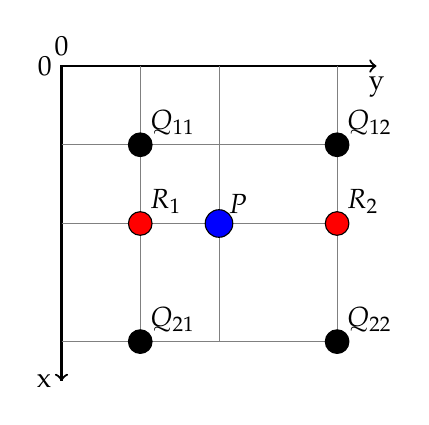
\begin{tikzpicture}[x=0.5cm,y=-0.5cm]
    
    % Draw the x-axis
    \draw[->,thick] (0,8) -- (0,0) -- (8,0) node[below] {y};
    % Draw the y-axis
    \draw[->,thick] (0,0) -- (0,8) node[left] {x};
    % Label the origin
    \node at (0,0) [left] {0};
    \node at (0,0) [above] {0};
    \foreach \x in {2,4,7}
    \draw[gray, very thin] (\x,0) -- (\x,7);
  \foreach \y in {2,4,7}
    \draw[gray, very thin] (0,\y) -- (7,\y);

    \foreach \Point/\PointLabel in {(7,4)/R_2,(2,4)/R_1}
    \draw[fill=red] \Point circle (0.3) node[above right] {$\PointLabel$};

    \foreach \Point/\PointLabel in {(2,2)/Q_{11}, (7,2)/Q_{12}, (2,7)/Q_{21}, (7,7)/Q_{22}}
    \draw[fill=black] \Point circle (0.3) node[above right] {$\PointLabel$};

    \foreach \Point/\PointLabel in {(4,4)/P }
    \draw[fill=blue] \Point circle (0.35) node[above right] {$\PointLabel$};

  \end{tikzpicture}

    \caption{Bilinear interpolation.}
    \label{fig:blinearInterpolation}
\end{figure}

\begin{minipage}{1\textwidth}
    \centering
    \begin{equation}
        v(x,y) = ax + by + cxy + d 
        \label{eq:bilinear}
    \end{equation}
    \begin{equation}
        f(R_{1}) \approx \frac{x_{2}-x}{x_{2}-x_{1}}f(Q_{11})+\frac{x-x_{1}}{x_{2}-x_{1}}f(Q_{21}) = R_{1}(x,y_{1})
    \end{equation}
    \begin{equation}
        f(R_{2}) \approx \frac{x_{2}-x}{x_{2}-x_{1}}f(Q_{12})+\frac{x-x_{1}}{x_{2}-x_{1}}f(Q_{22}) = R_{2}(x,y_{2})
    \end{equation}
    \begin{equation}
        f(P) \approx \frac{y_{2}-y}{y_{2}-y_{1}}f(R_{1})+ \frac{y-y_{1}}{y_{2}-y_{1}}f(R_{2}) = v(x,y)
    \end{equation}

    
\end{minipage}


\subsubsection{Histogram equalisation}
Another important aspect of preprocessing the frames is using Histogram equalization. This has the effect of increasing the contrast of the image. For this task Contras Limited Adaptive Histogram Equalization (CLAHE)\cite{clahe} is used. CLAHE is an Histogram Equalization method that has the benefit that it is adaptive to the local contrast of the image. This is very useful if the contrast of the image is not uniform. By using Histogram Equalization on the frames, noise is added to the image. This can be dealt with by using a low pass filter, like an Gaussian filter for example.

 Using a normal Histogram Equalization would lead to a loss of information in the region around the pupil and the iris. This is due to the fact that the contrast in this region is already very high. The CLAHE method splits the image into smaller blocks called "tiles"  and calculates the histogram on each block individualy and therefore does not lead to the same lose of important information at the pupil region. The CLAHE method is applied to the frames after they are converted to grayscale. The result of this step is shown in figure \ref{fig:clahe}. 

\begin{figure}[h]
    \centering
    \includegraphics[width=1\textwidth]{plots/clahe.png}
    \caption{Example of CLAHE an its effect on the histogram.}
    \label{fig:clahe}
\end{figure}
These are the parameters used for the CLAHE plots
\begin{python}
    clahe = cv2.createCLAHE(clipLimit=1.0, tileGridSize=(11,11))
\end{python}

\subsection{Edge Detection}
\subsubsection{Sobel Operators}
The Sobel Operators are used is a common algorithm for edge detection. It is a gradient calculation that uses a 3x3 differential kernel to calculate the gradient of the image. The Sobel gradient is calculated in x and y direction. The gradient in x and y direction are calculated by convolving the image with two different kernels. The image with gray values is defined as $f(x,y)$ and the kernels are defined as $k_x$ and $k_y$. Therefore the gradient is calculated as follows:
\begin{equation}
    \nabla f = \begin{bmatrix}
        G_x \\ G_y
    \end{bmatrix} = \begin{bmatrix}
        \frac{\partial f}{\partial x}  \\ \frac{\partial f}{\partial y}
    \end{bmatrix}
\end{equation}

\begin{center}
    \begin{minipage}{0.44\textwidth}
        \begin{equation}
            k_x = \begin{bmatrix}
                -1 & 0 & +1 \\
                -2 & 0 & +2 \\
                -1 & 0 & +1
            \end{bmatrix} 
        \end{equation}
    \end{minipage}
    \hfill
    \begin{minipage}{0.44\textwidth}
        \begin{equation}
            k_y = \begin{bmatrix}
                -1 & -2 & -1 \\
                0 & 0 & 0 \\
                +1 & +2 & +1
            \end{bmatrix} 
        \end{equation}
         
    \end{minipage}
\end{center}

    \begin{align}
        G_x(x,y) & = f(x,y) * k_x  = \sum_{s=-a}^{a} \sum_{t=-b}^{b} k_x(s,t) f(x+s,y+t) \\
        G_y(x,y) & = f(x,y) * k_y  = \sum_{s=-a}^{a} \sum_{t=-b}^{b} k_y(s,t) f(x+s,y+t)
    \end{align}

    $G_x(x,y)$ and $G_y(x,y)$ are the gradients in x and y direction. $f(x,y)$ is the image and $k_x$ and $k_y$ are the kernels. The kernels convolved with the image $f(x,y)$ and the result is the gradient magnitude in x and y direction. In other words the convolution of an image with $k_x$ or $k_y$ gives as result the change from pixel to pixel in x or y direction.
    In python the Sobel in x and y are calculated with the OpenCV Library for example:

    \begin{python}
    G_x = cv2.Sobel(img,cv2.CV_64F,1,0,ksize=3)
    G_y = cv2.Sobel(img,cv2.CV_64F,0,1,ksize=3)
    \end{python}
    The total gradient magnitude $G$ is calculated with this equation: 
    \begin{equation}
        G = \sqrt{G_x^2 + G_y^2}
        \label{eq:gradientmagnitude}
    \end{equation} 
    and the direction $\theta$ of the gradient is calculated with this equation:
    \begin{equation}
        \theta = \arctan{\frac{G_y}{G_x}}
        \label{eq:gradientdirection}
    \end{equation}
    The result of the convolution can be seen in figure \ref{fig:gradient} in chapter two. 

    \subsubsection{Canny Edge Detection} 
    The Canny Edge Detection is used to recieve single edge points form the gradient magnitude image.  
    This algorithm can summarized in four steps\cite{canny_edge}: 
    \begin{enumerate}
        \item Noise reduction, smoothing the image with a Gaussian filter
        \item Compute the gradient magnitude and direction
        \item Non-maximum suppression to the gradient magnitude image
        \item Use double thresholding and connectivity analysis to detect and link edges
    \end{enumerate}
\textbf{Step 1: Noise reduction} \\
The first step is to reduce noise from the input image. This is done by convolving the image with a low pass filter. For this task a Gaussian filter is used. The Gaussian filter is defined as:
\begin{equation}
    f_{filter}(x,y) = \frac{1}{2\pi\sigma^2}e^{-\frac{x^2+y^2}{2\sigma^2}}
\end{equation}
The Gaussian filter is then convolved with the image so smooth the image. 
\begin{equation}
    f_{smoothed}(x,y) = f(x,y) * f_{filter}(x,y)
\end{equation} 

\textbf{Step 2: Compute the gradient magnitude and direction} \\
The gradient magnitude is calculated with the equation \ref{eq:gradientmagnitude} and the gradient direction is calculated with the equation \ref{eq:gradientdirection}.

\textbf{Step 3: Non-maximum suppression} \\
The non-maximum suppression is used to thin the edges out, so that the edges are only one pixel wide. This can be achieved with an loop that goes over all edges and checks if the current pixel, belonging to the edge, is the local maximum in the direction of the $\pm $gradient vector. If that is the case the pixel is kept, otherwise it is set to zero. Because as already described in \ref{subsec:funda} the coordinate system is defined different. The gradient direction is in reference to the $x$ axis. 



\begin{figure}[h]
    \centering
        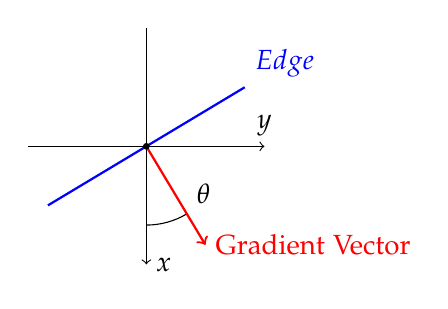
\begin{tikzpicture}[rotate=-90, scale= 0.5]
            % Draw the coordinate axes
            \draw[->] (-3,0) -- (3,0) node[right] {$x$};
            \draw[->] (0,-3) -- (0,3) node[above] {$y$};
            % Draw the first line
            \draw (2,0) arc (0:31:2)node[above right] {$\theta$};
            \draw[->,red,thick] (0,0) -- (2.5,1.5)node[right] {Gradient Vector};
            % Draw the angle marker
        
        ;
            % Draw the second line
            \draw[blue,thick] (1.5,-2.5) -- (-1.5,2.5)node[above right] {$Edge$};
            % Draw the origin
            \filldraw[black] (0,0) circle (2pt);
        \end{tikzpicture}
        \caption{Definition of the gradient direction}
        \label{fig:Definition_grad}
\end{figure}
Because an image is quantized, this also means that $\theta$ needs to be quantized to four directions to evaluate their neighbors. 

\begin{figure}[h]
    \centering
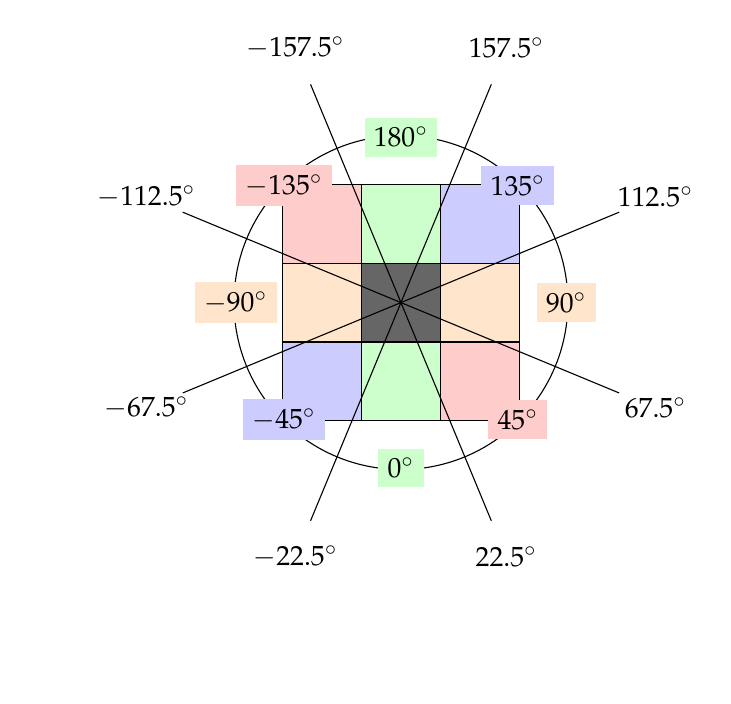
\begin{tikzpicture}[x=1cm,y=1cm]
    % Draw the grid
    \draw (0,0) grid (3,3);
     % Draw unit circle around grid

    % Fill the center pixel with light gray
    \filldraw[fill=blue!20] (0,0) rectangle (1,1);
    \filldraw[fill=blue!20] (2,2) rectangle (3,3);
    \filldraw[fill=orange!20] (0,1) rectangle (1,2);
    \filldraw[fill=orange!20] (2,1) rectangle (3,2);
    \filldraw[fill=red!20] (0,3) rectangle (1,2);
    \filldraw[fill=red!20] (2,0) rectangle (3,1);
    \filldraw[fill=green!20] (1,0) rectangle (2,1);
    \filldraw[fill=green!20] (1,2) rectangle (2,3);
    \filldraw[fill=black!60] (1,1) rectangle (2,2);


    \draw (1.5, 1.5) circle [radius=2.12];
    % Mark angles in 45° steps
    \foreach \ang in {157.5,112.5,67.5,22.5,-22.5,-67.5,-112.5,-157.5} {
        \draw (\ang-90:3.5) ++(1.5,1.5) node [fill=white] {$\ang^\circ$};
        \draw (\ang-90:3) ++(1.5,1.5) -- (1.5,1.5) ;

    }
    \foreach \ang in {0,180} {
        %\draw[thick,green] (\ang-90:2.3) ++(1.5,1.5) -- (1.5,1.5) ;
        \draw (\ang-90:2.1) ++(1.5,1.5) node [fill=green!20] {$\ang^\circ$};

    }

    \foreach \ang in {-45,135} {
        %\draw[thick,blue] (\ang-90:2.3) ++(1.5,1.5) -- (1.5,1.5) ;
        \draw (\ang-90:2.1) ++(1.5,1.5) node [fill=blue!20] {$\ang^\circ$};


    }
    \foreach \ang in {-90,90} {
        %\draw[thick,orange] (\ang-90:2.3) ++(1.5,1.5) -- (1.5,1.5) ;
        \draw (\ang-90:2.1) ++(1.5,1.5) node [fill=orange!20] {$\ang^\circ$};


    }
    \foreach \ang in {45,-135} {
        %\draw[thick,red] (\ang-90:2.3) ++(1.5,1.5) -- (1.5,1.5) ;
        \draw (\ang-90:2.1) ++(1.5,1.5) node [fill=red!20] {$\ang^\circ$};


    }

         % Add a tick at 45 degrees

\end{tikzpicture}
  \caption{Quantization of the gradient direction}
  \label{fig:non_max}
\end{figure}
This leads following quantizations: 
\begin{equation}
    \theta_q = \begin{cases}
    90, & \text{if } 67.5^\circ < \theta \leq 112.5^\circ \, \vee \, -112.5^\circ < \theta \leq -67.5^\circ \\
    -45^\circ, &\text{if }22.5^\circ < \theta \leq 67.5^\circ \, \vee \, -157.5^\circ < \theta \leq -112.5^\circ \\
    +45^\circ, &\text{if }112.5^\circ <\theta \leq 157.5^\circ \, \vee \, -67.5^\circ < \theta \leq -22.5^\circ \\
    0^\circ, &\text{if }-22.5^\circ <\theta \leq 22.5^\circ \, \vee \, -157.5^\circ < \theta \leq 157.5^\circ \\
\end{cases} 
\label{eq:quantization_d}
\end{equation}
It is important to note that when following the gradient direction, the two neighboring pixels are used to evaulate the gradient magnitute maximum. This is shown in figure \ref{fig:non_max} and \ref{fig:neighbors}.
If the gradient is maximal at the current pixel at $(x,y)$, meaning it is a local maximum in the previous defined neighborhood in respect to the gradient direction, the value of the pixel is written into $g_n(x,y)$, otherwise it is set to zero $g_n(x,y) = 0$. This is called non-maximum suppression. Therefore $g_n(x,y)$ contaians only the thinned edges.  

\begin{figure}[ht]
    \centering
    \begin{subfigure}[b]{0.23\textwidth}
        \centering
        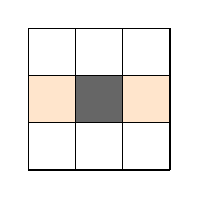
\begin{tikzpicture}[scale=0.6]
            \draw (0,0) grid (3,3);
            \filldraw[fill=orange!20] (0,1) rectangle (1,2);
            \filldraw[fill=orange!20] (2,1) rectangle (3,2);
            \filldraw[fill=black!60] (1,1) rectangle (2,2);
        \end{tikzpicture}
        \caption{Neighbors: 90°}
        \label{fig:n90}
    \end{subfigure}%
    \begin{subfigure}[b]{0.23\textwidth}
        \centering
        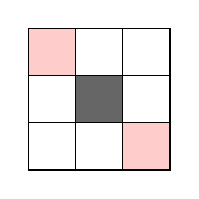
\begin{tikzpicture}[scale=0.6]
            \draw (0,0) grid (3,3);
            \filldraw[fill=red!20] (0,3) rectangle (1,2);
            \filldraw[fill=red!20] (2,0) rectangle (3,1);
            \filldraw[fill=black!60] (1,1) rectangle (2,2);
        \end{tikzpicture}
        \caption{Neighbors: 45°}
        \label{fig:n45}
    \end{subfigure}%
    \begin{subfigure}[b]{0.23\textwidth}
        \centering
        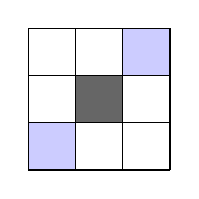
\begin{tikzpicture}[scale=0.6]
            \draw (0,0) grid (3,3);
            \filldraw[fill=blue!20] (0,0) rectangle (1,1);
            \filldraw[fill=blue!20] (2,2) rectangle (3,3);
            \filldraw[fill=black!60] (1,1) rectangle (2,2);
        \end{tikzpicture}
        \caption{Neighbors: -45°}
        \label{fig:nn45}
    \end{subfigure}%
    \begin{subfigure}[b]{0.23\textwidth}
        \centering
        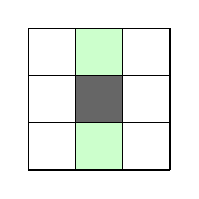
\begin{tikzpicture}[scale=0.6]
            \draw (0,0) grid (3,3);
            \filldraw[fill=green!20] (1,0) rectangle (2,1);
            \filldraw[fill=green!20] (1,2) rectangle (2,3);
            \filldraw[fill=black!60] (1,1) rectangle (2,2);
        \end{tikzpicture}
        \caption{Neighbors: 0°}
        \label{fig:n0}
    \end{subfigure}
    \caption{The gradient magnitude is evaluated in the direction of the gradient.}
    \label{fig:neighbors}
\end{figure}

  

\textbf{Step 4: Double thresholding and connectivity analysis} \\
After Step 3, $g_n(x,y)$ still shows edges that can be thicker than one pixel. $g_n(x,y)$ is then thresholded with a high an low threshold (hysteresis thresholding) creating two images: 
\begin{equation}
    g_{low}(x,y) = \begin{cases}
    g_n(x,y), & \text{if } g_n(x,y) \geq T_{low} \\
    0, &\text{otherwise}
\end{cases}
\end{equation}
\begin{equation}
    g_{high}(x,y) = \begin{cases}
    g_n(x,y), & \text{if } g_n(x,y) \geq T_{high} \\
    0, &\text{otherwise}
\end{cases}
\end{equation}
Because two different thresholds were used, there is still overlap between $g_{low}$ and $g_{high}$. All non zero pixels in $g_{high}$ are considered strong edge pixels. To recieve all weak edge pixels, the strong edge pixels are substracted from $g_{low}$. The remaining pixels are considered weak edge pixels.
\begin{equation}
    g_{weak}(x,y) = g_{low}(x,y) - g_{high}(x,y)
\end{equation}
Next step is to connect the weak edge pixels to the strong edge pixels. This is done by checking the 8-neighborhood of each strong edge pixel. If there is a weak edge pixel in the neighborhood, it is considered a strong edge pixel. This is done until no more weak edge pixels are found. The result is a binary image $g_{final}(x,y)$ containing all edges. But this still does not return a one pixel thick edge. 

To solve this the edges are passed on an edge-thinning algorithmus. Let's define the edges as set A and B as a structuring element. 
The equation for thining then becomes: 
\begin{equation}
    A \otimes   B = A - (A \circledast B)
\end{equation}
Where $\otimes$ is the thinning operator, $\circledast$ is the dilation operator.
\chapter{Algorithm Implementation}
In this chapter some of the algorithm in the theory chapter are combined, tested and evaluated. The goal is to find the most robust combination of algorithms to detect the pupil even in a very demanding data set like the LPW. The LPW data set is already discussed in its chapter and will not be discussed here again. In general the evaluation can be split up into two part. The first part is localization of the pupil and second part is finding the pupil ellipse. The importance of the localization is that with the information of the location of the pupil it is possible to create a region of interest (ROI). This has the benefit that in the second part the image size is already decreased and additional noise can be even more limited. Also the computational effort is reduced because the image size is smaller. Important to note is, that all algorithms make the basic assumption, that the pupil is always visible. So blinking is not counted as a failure and excluded of the evaluation if possible. For detecting blinking, other algorithms need to be used to preprocess every frame and detect if the eye is closed or not. 


\section{Localization}
For the localization mainly thresholding, edge detection and haar-like features were implemented and can now be evaluated. To make thresholding more flexible a semi adaptive algorithm was created to choose the best fitting threshold value. The histogram is used to determine the highest peak in the low intensity range. This value is then used to threshold the image. 
\begin{equation}
    t = \text{argmax} \{h(i) | i \in [0,255]\}
\end{equation}
With $h(i)$ being the histogram of the image. The threshold value is then used to calculate a range for using double thresholding to extract the pupil. The image is modified by setting all values below and above the threshold value to 0. 
\begin{equation}
    f(x,y)= \begin{cases}
        0 &iff \quad I(x,y) < t-35 \quad \text{or} \quad I(x,y) > t+25 \\
        I(x,y) &otherwise
    \end{cases}
\end{equation}
\subsection{Thresholding}
Whereas the under limit of the threshold is set lower than the higher limit. This derives from testing and can be concluded, that the probability that the pixels with lower intensity values belongs to the pupil is higher than the probability that the pixels with higher intensity values belong to the pupil. In a environment with almost no noise and most important no reflections this approach works very well. But as also already mentioned in the theory section, reflections lead to a less higher peak in the histogram and the possibility exist that the threshold value has no peak in the lower values range and therefore leads to a faulty result that can not be used to create an ROI or use it with edge detection to find the boundary of the pupil. Also it is important to note that with this thresholding approach the mask created is not a binary mask but a mask with values between $[t-35, t+25]$. But the possibility to use the binary mask still exist and the all contours found in this threshold range are evaluated by their circularity and similarity to an ellipse. The best fitting contour is then used to create the ROI or ellipse fit directly to find the ellipse parameters. 
[RESULTS]
This method works in a environment with almost no noise flawless, it is has benefit to reach the goal in almost realtime but in with the LPW data set it is keen to strugle with most of the conditions and is therefore not usefull for the LPW data set.

\subsection{Edge detection}
Edge detection is strongly effected by noise and therefore the preprocessing is key for useful results. Every frame undergoes the same preprocessing as in the other algorithms but a gaussian blur is used additionally to smooth fast changing intensity regions out.  Even though the gaussian blur is used, there is still information missing that is covered by noise. The edges are detected but the same problem as with thresholding arises here. By using Sobel and than the Canny edge detection the results are useful in a environment with almost no noise but as already said, LPW is known for its noise and reflections. Canny edge detection needs two threshold parameters to work properly and also here arises the problem that these parameters need to be adaptive to the environment which can be tricky. 
[RESULTS]

\subsection{Haar-like features}
The Haar-like feature is the approach that is proposed by this thesis to find the region of interest. It has the best detection rate of all approaches tested on the LPW data set and is therefore the best approach to find the ROI. The Haar-like feature is constructed as described in the theory part and is shown in \ref{fig:haar_pupil}. 
The calculation of the feature vector is done by using the integral image and is done 3 times with variating Radius $r$ all feature vectors are then compared and the location of the highest response is returned as a point that lies on the pupil. 

\begin{figure}[h]
    \centering
    \begin{subfigure}{0.5\textwidth}
        \centering
        \includegraphics[width=0.9\linewidth]{plots/results/originalbest.png}
        \caption{Original Frame}
    \end{subfigure}%
    \hfill
    \begin{subfigure}{0.5\textwidth}
        \centering
        \includegraphics[width=0.9\linewidth]{plots/results/responsehaarbest.png}
        \caption{feature vector, blue is the best response}
    \end{subfigure}%
 
    \caption{Feature vector for pupil detection}
    \label{fig:limit_haar}
\end{figure}

The stronges response lies then within the pupil and the location is then used to create a ROI. In this case a ROI of $110 x 110$ was the norm but depending on the rescaling of the frames this can be adapted. Important to note is, that the returned point in the pupil is not given to be in the center. This in an important fact when choosing the size of the ROI that is created. 
But this approach is still not perfect and even though it can handle noise really good, there are limits to the amount of noise until the algorithm fails. Also the algorithm is not able to detect the pupil when the eye is closed.

\begin{figure}[h]
    \centering
    \begin{subfigure}{0.5\textwidth}
        \centering
        \includegraphics[width=0.9\linewidth]{plots/results/originalworst.png}
        \caption{Extreme noise example}
    \end{subfigure}%
    \hfill
    \begin{subfigure}{0.5\textwidth}
        \centering
        \includegraphics[width=0.9\linewidth]{plots/results/responsehaarworst.png}
        \caption{feature vector result with best response}
    \end{subfigure}%
 
    \caption{Limits to the Haar-like feature approach}
    \label{fig:limit_haar}
\end{figure}
The problem with the LPW data set is, that it is so versatile and the conditions change during the recording. This makes it hard to find an approach that can adapt to all the conditions and still perform well in a given time interval. The implementation can still be improved and sped up, in the Haar-like feature the following libraries were used to speed up the algorithm: 

\begin{python}
from concurrent.futures import ThreadPoolExecutor
from numba import njit
    \end{python}
ThreadPool Executor makes it possible to use multithreading and njit compiles the sliding window over the integral image of the Haar-like feature to machine code for more efficient calculation.

\section{Ellipse parameter estimation}
In the second part of an pupil detection algorithm it is necessary to make use of the informations from the first part and build on this foundation and find the five ellipse parameter: center: $(x,y)$, axis: (major, minor) and angle. The LPW has labels for the center only of the pupil and therefore only the center can be used to evaluate the performance of the algorithms. A second evaluation has to be done manually by inspecting the fit of the ellipse to the pupil. This is hard to evaluate with numerical methods and the result needs therefore to be taken with a grain of salt. In this section 4 different algorithms will be discussed and evaluated: The OpenCV ellipse fit based on contours (binary thresholding), ACWE with OpenCV Ellipse fit, ACWE combined with RANSAC, and Canny edge detection with OpenCV Ellipse fit. 

\subsection{Thresholding and OpenCV ellipse fit}
The benefit of this method is that it can almost run in realtime and still perform well in certain frames where the noise is low and the pupil is clearly visible. But as already mentioned in the localization part, this method is not robust enough to handle the LPW data set. The thresholding is done with the same approach as in the localization part and the binary mask is then used to find the contours. The contours are then evaluated by their circularity and similarity to an ellipse. The best fitting contour is then used to fit an ellipse with the OpenCV ellipse fit function. The OpenCV ellipse fit function is based on the least square method and therefore very robust and fast. The ellipse fit is then evaluated by the center and the distance to the ground truth center. The problem with least square method is, lies in the definition itself. Because the method tries to find an ellipse that minimizes the distance from every point on the boundary of the binary mask to the ellipse curve. When the pupil is partially covered by noise, the contour does not match the original shape of the pupil and does not represent the total pupil boundary. Using least square method in this case leads to a faulty ellipse fit where the result is not usable. The amount of outliers is to high and the ellipse fit is not accurate enough because there is information missing. 
\begin{figure}[h]
    \centering
    \begin{subfigure}{0.3\textwidth}
        \centering
        \includegraphics[width=0.9\linewidth]{plots/results/roi_text_resutls.png}
        \caption{ROI}
    \end{subfigure}%
    \hfill
    \begin{subfigure}{0.3\textwidth}
        \centering
        \includegraphics[width=0.9\linewidth]{plots/results/roi_binary_ellipse.png}
        \caption{Binary thresholding}
    \end{subfigure}%
    \hfill
    \begin{subfigure}{0.3\textwidth}
        \centering
        \includegraphics[width=0.9\linewidth]{plots/results/roi_result_binary_ellipse.png}
        \caption{OpenCV Ellipse fit}
    \end{subfigure}%
    \caption{Binary thresholding with OpenCV ellipse fit}
    \label{fig:binary_threshold_ellipse_fit}
\end{figure}

\subsection{Canny edge detection with OpenCV ellipse fit}


\subsection{ACWE with OpenCV ellipse fit}


\subsection{ACWE combined with RANSAC}


\chapter{Proposal}
\label{chap:proposal}
\section{Proposed Algorithm}
After intensive research and analysis, the algorithm proposed for pupil detection consist of the following steps: 
\begin{enumerate}
    \item \textbf{Preprocessing:} The image is converted to grayscale, and then the histogram equalization method CLAHE is used to improve the image's contrast.
    \item \textbf{Haar-like features:} From the image the response matrix is calculated using the Haar-like feature for pupil detection proposed by \ref{subsec:haar}. The response matrix is then used to find the strongest response in the image, and this point is considered to be inside the pupil area. 
    \item \textbf{ACWE} The active contour without edges algorithm is applied to the image with the point returned by the Haar-like feature detection as center of the initial contour. ACWE then returns the contour of the pupil.
    \item \textbf{RANSAC} The RANSAC algorithm is applied to the mask returned by the ACWE algorithm. Iterates over the mask contour and fits a circle to a random subset of the contour points. RANSAC returns the circle with the best fit.
\end{enumerate}
\chapter{Results}
In this chapter the proposed algorithm is evaluated on the LPW data set and numerical results are presented, followed by a discussion of the results. 
\section{Evaluation}

\chapter{Conclusion}
\label{chap:conclusion}
\section{Summary}


%\chapter{Theory}

In this chapter will take a look at commonly used algorithms in image processing for edge detection, identifyig areas of interest and refining them. 
We discuss those algorithms first in theory and then show it's use case in detecting the iris of an human eye. 

To show the nature of the algorithm, the same preprocessed image is used and therefore it is possible to showcase the results and compare the algorithms in a later chapter
\section{Algorithms}




\subsection{Preprocessing}
To be able to compare the different approaches, it is important to define the used algorithms that lead to the wanted result.
An image taken has to be preprocessed first. The idea behind this step is to create a common ground for narrowing the deviation of the images down, so that the algorithms are 
able to recreate the same result over span of different images.

\subsubsection{Histogram matching}
The algorithms are trimmed to a specific Histogram to work the best. Therefore all Images have to be preprocessed. To fullfil this requirement, Histogram matching is done. In the first step
we take a look at the histogram used to match the others onto. 

\section{Gaussian blur}
The idea behind using a Gaussian blur on a Image first is to minimize unnecessary information in to be processed image. By using the gaussian blur the image loses details and 
this increases the chance to find the main edges in the image, finding the outline of the iris. 


Dummy text.

\subsection{Definition RANSAC}

Dummy text.


\section{Canny Edge Detection}

Dummy text.

\subsection{Definition Canny Edge Detection}

Dummy text.

\section{Active Contur}

Dummy text.

\subsection{Definition Active Countur}

Dummy text.

\subsubsection{Example Subsubsection}

Dummy text.

\paragraph{Example Paragraph}

Dummy text.

\subparagraph{Example Subparagraph}

Dummy text.

%\input{rules}
%\input{typography}
%\input{sections}

\appendix

\chapter{Appendix}
\label{appendix}
\section{Choosing the right model}
Depending on the level of noise different algorithms can be considered. Here only algorithms that are implemented in the thesis are considered. There are even more algorithms that could be used for object sedimentation for example MSER or Machine Learning. 
\subparagraph{Low noise}
If there is almost no noise in the image, meaning the pupil is all the time clearly visible and no reflections in the pupil area, it is possible to use the Haar-like feature to localize the pupil. Create a ROI and then use the intensity Value of the pixel with the best response from the Haar-Like Feature to get a threshold value. Then create a binary mask and inspect all contours in the ROI and choose the contour with the best circularity and similarity to an ellipse. Use OpenCV ellipse fit to retrieve the ellipse parameters. This approach is very fast and accurate in low noise conditions and can almost run in realtime. 
\subparagraph{Medium noise / High noise}
Here it becomes more tricky to choose the right mode. In general the more noise is introduced the more robust the algorithm has to be. This comes with the cost of speed. Here the proposed algorithm should be used to extract the pupil parameters. 

\section{Code}
All the code can be found on github under: \url{https://github.com/parisj/Algorithms_Eye_Detection}. The code is implemented in python and for the packages used, take a look a the requirement.txt file

\backmatter

\bibliographystyle{unsrt}
\bibliography{refs}

\includepdf[pages={-}]{declaration-originality.pdf}

\end{document}
